\begin{figure*}[t!]
\begin{center}\footnotesize
	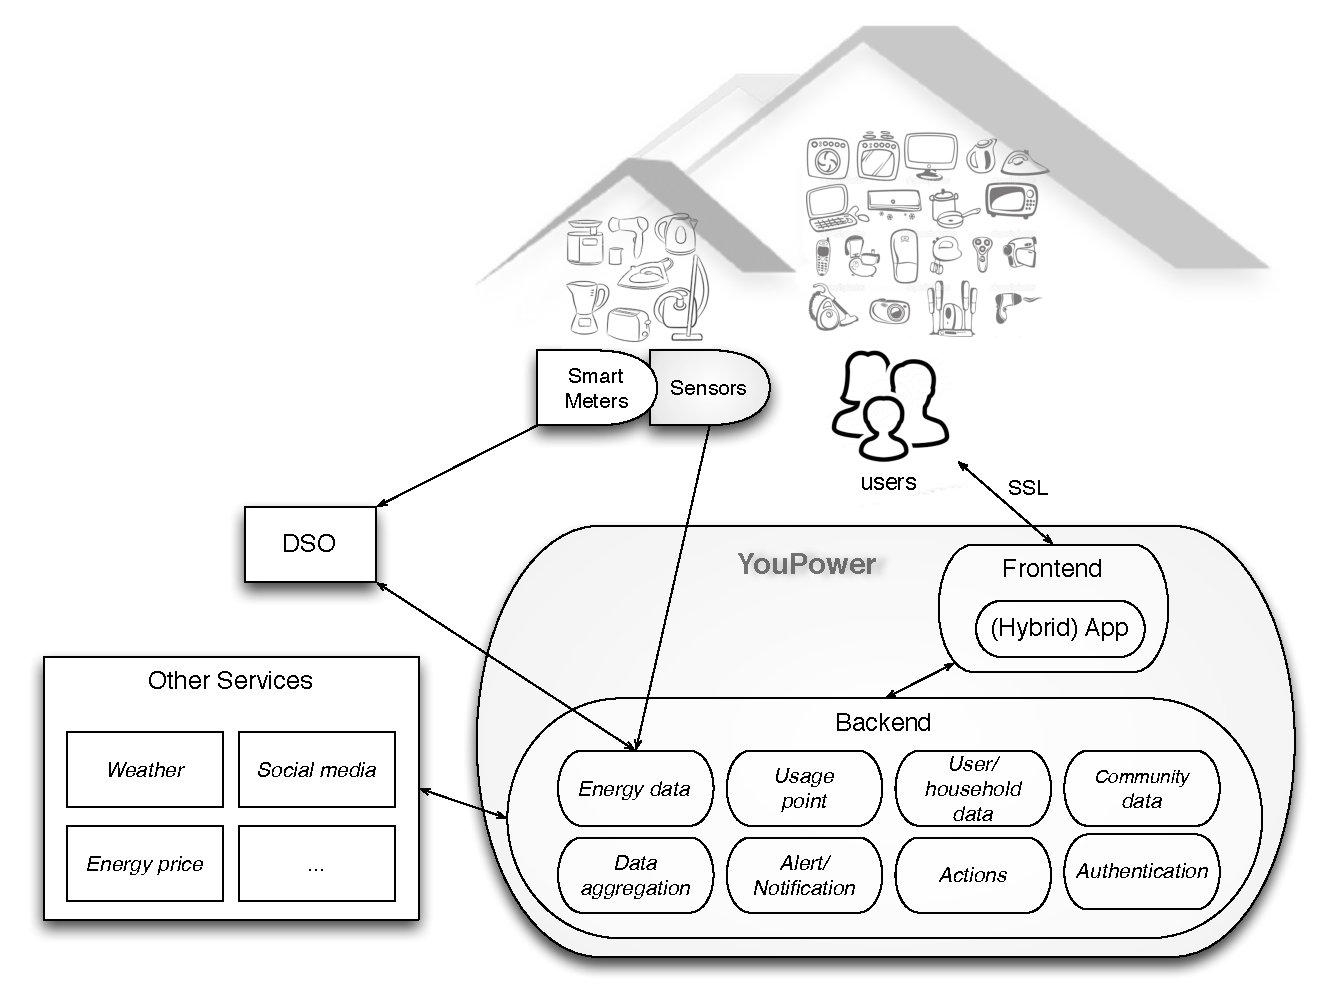
\includegraphics[width=.7\textwidth]{img/civis_platform_overview.pdf}\\
	DSO (Distribution System Operators),  SSL (Secure Sockets Layer)
	\caption{YouPower system overview}\label{fig:platform}
\end{center}
\end{figure*}

\section{\uppercase{State of the Art}}

\noindent Prior to designing YouPower, we first review existing proposals for social platforms in the context of power grids. Second, we summarize the findings about success of different consumer behavior change interventions and strategies. One of the repeatedly reported drawbacks of different solutions aiming to involve consumers is a lack of their sustained use \cite{edward2015review}. Iterative and lean design process that we adopt is suggested as a promising approach to tackle this problem \cite{schwartz2014people}.

Weiss et al.~\cite{weiss2012powerpedia} developed a smartphone community platform, PowerPedia. The platform works in connection with smart meters and enables users to identify and upload their own appliance-level consumption statistics. After upload, the users can compare their appliance consumption with other users. The platform was evaluated in a lab setting and the test users rated favorably social comparison features and appliance level statistics.

Community Monitor \cite{dillahunt2014understanding} is a social energy app deployed on tablets that was tested in two distinct communities for 4-10 months. The app featured leaderboard, message board and shared actions ("ways to save"). The findings from the trial revealed importance of environmental, social and cultural context for the app use. For instance, the existence of common spaces for community members to interact and knowledge of other users supported the app use. On the other hand, shorter length of residence or rented apartment negatively affected the engagement. Community Monitor did not manage to engage users around the message board feature.

Petkov et al.~\cite{petkov2011motivating} delve more into the details of comparative feedback. Their findings confirm importance of comparisons to similar users in terms of energy consumption and neighbors. However, if the competition features are included, then the users preferred to compete with the people whom they actually know and especially with their friends. 

X Considering the analytical frames and the CIVIS use cases, we chose a set of platform features and translated those into three self-contained and composable parts to be included in the CIVIS (front-end) application (hereinafter abbreviated as CIVIS app): 
%\begin{enumerate}
%\item \nameref{sect:tips}
%\item \nameref{sect:brf}
%\item \nameref{sect:load_shifting}
%\end{enumerate}



With peer review results and users' feedback on the design, adaptations and changes are made to suit user needs and to achieve the CIVIS research goal. 
In general, the application aims to enhance users' energy know-how through action suggestions that are implementable in everyday life, engage users in energy communities with understandable and actionable information and feedback, and facilitate community interaction and self-teaching by means of group discussions.
%

Given the time and resource constraints, the app can not be developed all-in-one cross-platform (for phones, tablets and computers). We chose to design the front-end as a mobile app. This means that the app design has layouts and user interactions that suit (small) phone screens. %The consideration is multi-fold. 
Western Europe has a large mobile phone internet user base\footnote{
Between 2013 and 2017, the penetration rate of mobile phone internet users among mobile phone users will rise from 49.0\% to 77.8\%. See more at:\url{ http://www.emarketer.com/Article/Nearly-Half-of-Western-Europeans-Will-Use-Mobile-Web-This-Year/1010510\#sthash.AaVfsqIU.dpuf}}. Many surveys show that mobile apps have advantages such as creating deeper user engagement, easy sharing, among others\footnote{\url{https://infomedia.com/blog/the-advantages-of-mobile-apps/}, \url{https://econsultancy.com/blog/62326-85-of-consumers-favour-apps-over-mobile-websites/}}. This makes mobile app a good choice given the goal of the CIVIS platform. Once developed, mobile apps can also be more easily transformed to web browser versions, while the reverse is more difficult. The back-end of the CIVIS platform will remain mostly the same independent of the front-end alternatives. 